
\resetcounters

\bibliographystyle{asp2010}

\markboth{Yamauchi}{2MASS Catalog Server Kit Version 2.1}

\title{2MASS Catalog Server Kit Version 2.1}
\author{Chisato~Yamauchi
\affil{Astronomy Data Center,
    National Astronomical Observatory of Japan,
    2-21-1 Osawa, Mitaka, Tokyo, 181-8588, Japan}
}

\aindex{Yamauchi, C.}

\begin{abstract}
The 2MASS Catalog Server Kit is \ssindex{software!open source}open source software for use in easily constructing a high performance search server for important astronomical catalogs. This software utilizes the \ssindex{software!open source}open source RDBMS \ssindex{databases!Postgres}PostgreSQL, therefore, any users can setup the database on their local computers by following step-by-step installation guide. The kit provides highly optimized stored functions for positional searchs similar to \ssindex{surveys!Sloan Digital Sky Survey(SDSS)}SDSS SkyServer. Together with these, the powerful\ssindex{databases!querylanguage!SQL} SQL environment of \ssindex{databases!Postgres}PostgreSQL will meet various user's demands.

We released 2MASS Catalog Server Kit version 2.1 in 2012 May, which supports the latest\ssindex{catalogs!individual!WISE} \ssindex{observatories!space-based!WISE}WISE All-Sky catalog (563,921,584 rows) and 9 major all-sky catalogs. Local databases are often indispensable for observatories with unstable or narrow-band networks or severe use, such as retrieving large numbers of records within a small period of time. This software is the best for such purposes, and increasing supported catalogs and improvements of version 2.1 can cover a wider range of applications including advanced calibration system, scientific studies using complicated\ssindex{databases!querylanguage!SQL} SQL queries, etc.

Official page: {\tt http://www.ir.isas.jaxa.jp/\~{}cyamauch/2masskit/}
\end{abstract}


\section{Purpose}

One of the most important points of 2MASS Catalog Server Kit \citep{yam_2011a} is that users directly input\ssindex{databases!querylanguage!SQL} SQL statements into the database server.\ssindex{databases!querylanguage!SQL} SQL has powerful flexibility in the programming interfaces for searching and manipulating tables, therefore, 2MASS Kit can be adapted to a wide variety of purposes.

Typical use cases will be 1) Astrometric and flux calibration at observatories with unstable or narrow-band networks, and 2) Severe use, such as retrieving large numbers of entries or complicated\ssindex{databases!querylanguage!SQL} SQL queries for calibration, scientific studies, etc. Actually, the \ssindex{observatories!Earth-based!CFHT}CFHT observatory and some Japanese institutes/observatories employ our 2MASS Kit. \ooindex{2masskit, ascl:1303.016}

\section{Supported Catalogs}

2MASS Kit version 2.1 supports 10 major all-sky catalogs in optical and infrared bands:
\begin{center}
\begin{tabular}{ll}
\hline
\small{ \ssindex{catalogs!individual!2MASS}2MASS PSC (470,992,970 rows) }   &    \small{    GSC-2.3.2 (945,592,683 rows)} \\
\small{\ssindex{catalogs!individual!WISE} \ssindex{observatories!space-based!WISE}WISE All-Sky (563,921,584 rows)} &       \small{UCAC3 (100,766,420 rows)} \\
\small{ USNO-B1.0 (1,045,175,762 rows)} &    \small{   PPMXL (910,468,710 rows) }\\
\small{ AKARI IRC PSC (870,973 rows)  }  &    \small{   \ssindex{catalogs!individual!Tycho-2 stellar catalog}Tycho-2 (2,539,913 rows) }\\
\small{ AKARI FIS BSC (427,071 rows)  }  &    \small{   IRAS PSC (245,889 rows) }\\
\hline
\end{tabular}
\end{center}
\ssindex{observatories!space-based!WISE}WISE 3-Band Cryo Release (261,418,479 rows) and UCAC4
will be supported in the near future.


\section{Optimized Search Functions}

Users can instantly use 2MASS Kit's high-speed positional search implemented by reasonable database design and high-level tuning of indices and stored functions. 2MASS Kit has three types of stored functions for positional searches: 1) Radial Search in J2000, Ecliptic,\ssindex{astronomy!Galactic} Galactic, and B1950 coordinate systems, 2) Box Search in J2000, Ecliptic,\ssindex{astronomy!Galactic} Galactic, and B1950 coordinate systems, and 3) Rectangular Search in the J2000 coordinate system.


\section{System Requirements}

Installing 2MASS Kit requires 64-bit or\ssindex{computing!architecture} 32-bit OS on which \ssindex{databases!Postgres}PostgreSQL-8.4 (or later) server works. Three Tbyte of hard drive has to be prepared to register all supported catalogs. Of course, you can also install only specific catalogs. Required disk space for each catalog is shown in 2MASS Kit Web page.

An external USB-2.0 hard drive can be used for typical searches, but we recommend a system with RAID10 and/or SSD for severe use. In 2MASS Kit database, each table/index is registered in one of six table spaces (each resides in a separate directory) for flexible tuning. This allows only the essential parts to be easily moved onto fast devices.


\section{How Useful is it?}

We show actual\ssindex{databases!querylanguage!SQL} SQL statements used on the 2MASS Kit database and their results. We recommend you to try the following examples, changing the arguments of stored functions, to know the real speed of our database.

\begin{verbatim}
-- An SQL statement to perform a radial search of 2MASS with J2000:
SELECT * FROM fTwomassGetNearbyObjCel('j2000', 266,-29, 0.2);
\end{verbatim}

{\small
\begin{verbatim}
   objid   |    lon     |    lat     |     distance      
-----------+------------+------------+-------------------
 684105609 | 265.999015 | -29.002653 | 0.167362064774342
 684575681 | 266.002656 | -28.999596 | 0.141471788449169
\end{verbatim}
}

\begin{verbatim}
-- Join the return value from the function to the Main Table:
SELECT o.ra, o.dec, o.j_m, o.h_m, o.k_m, n.distance
FROM fTwomassGetNearbyObjEq(266, -29, 0.2) n, Twomass o
WHERE n.objid = o.objid;
\end{verbatim}

{\small
\begin{verbatim}
     ra     |    dec     |  j_m   |  h_m   |  k_m   |     distance     
------------+------------+--------+--------+--------+-------------------
 265.999015 | -29.002653 | 12.502 | 11.488 | 10.551 | 0.167362064774342
 266.002656 | -28.999596 | 14.579 | 11.091 |  9.283 | 0.141471788449169
\end{verbatim}
}

Shown in next example, 2MASS Kit provides stored functions for coordinate conversion. Some\ssindex{computer languages!C} C functions of WCSTools \citep{min_2006} are used to implement them. \ooindex{WCSTools, ascl:1109.015}

\begin{verbatim}
-- To display positions in sexagesimal and in Galactic coordinate:
SELECT fDeg2LonStr(o.ra) as ra, fDeg2LatStr(o.dec) as dec, 
       fJ2L(o.ra,o.dec) as l, fJ2B(o.ra,o.dec) as b
FROM fTwomassGetNearbyObjEq(266, -29, 0.2) n, twomass o
WHERE n.objid = o.objid;
\end{verbatim}

{\small
\begin{verbatim}
     ra      |     dec     |        l         |         b         
-------------+-------------+------------------+-------------------
 17:43:59.76 | -29:00:09.6 | 359.757732609713 | 0.268108804975495
 17:44:00.64 | -28:59:58.5 | 359.762004949764 | 0.266998167472491
\end{verbatim}
}

\begin{verbatim}
-- Search elongated region along Galactic plane:
SELECT count(*) 
FROM fTwomassGetNearbyObjFromBoxCel('galactic',0,0,600,1);
\end{verbatim}

{\small
\begin{verbatim}
 count 
-------
 85410
\end{verbatim}
}

{\small
\begin{verbatim}
-- Perform a radial search of IRAS and a cross-id between 2MASS and
-- returned result of IRAS.  Using SSD is recommended for performance:
SELECT r.ra as ra_iras, r.dec as dec_iras,
       p.ra as ra_2mass, p.dec as dec_2mass,
       fDistanceArcMinEq(r.ra,r.dec,p.ra,p.dec) as distance
FROM (
 SELECT o.*
 FROM fIrasGetNearbyObjEq(180,2,60) n, Iras o
 WHERE o.objid = n.objid
) r
LEFT JOIN Twomass p
ON fTwomassGetNearestObjIDEq(r.ra,r.dec, 1.0) = p.objID;
\end{verbatim}
}

{\small
\begin{verbatim}
  ra_iras   | dec_iras |  ra_2mass  | dec_2mass |      distance      
------------+----------+------------+-----------+--------------------
 179.849487 | 1.827165 | 179.849741 |  1.826719 | 0.0307915522123298
 180.673096 | 1.977994 | 180.675986 |  1.976742 |  0.188877689977676
 179.247971 | 2.409427 | 179.242712 |  2.412174 |  0.355745637503231
\end{verbatim}
}


\section{Database Design}

\subsection{Spatial Indexing}

Neither \ssindex{libraries!HTM}\ssindex{methods!indexing!Hierarchical Triangular Mesh (HTM)}HTM \citep{kun_2000} nor \ssindex{libraries!HEALPix}HEALPix \citep{gor_2005} are used. To enable high-speed radial and box searches, we use a composite index on unit vectors of positions ({\tt cx}, {\tt cy}, {\tt cz}) and select entries with the following procedure: 1) Catch objects within a cube (or multiple cubes) using index scan on ({\tt cx}, {\tt cy}, {\tt cz}), and 2) Select objects within the strict search circle (or box) on the celestial sphere from the result of step 1. Figure 2 in \citet{yam_2011a} shows the concept of our radial search that uses $x$$y$$z$ coordinate for the database index.

The feature of our algorithm is that it requires almost no calculation before executing the index scan, and the efficiency is quite high for a small search radius. In addition, we do not have to implement special processing for the polar singularity.

\subsection{Special Design for Huge Catalogs}

\begin{figure}[t]
\centering
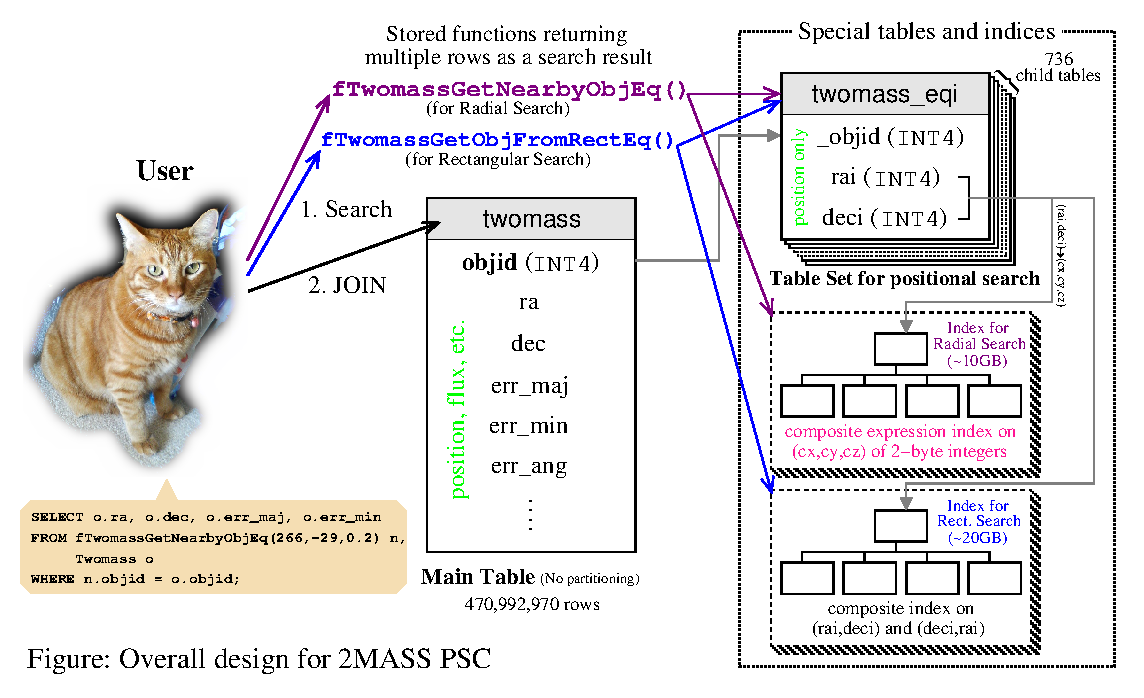
\includegraphics[width=0.75\textwidth]{part10/Yamauchi_P35/db_design.eps}
\end{figure}

If we apply a straightforward implementation for huge catalogs, two problems will arise: 1) Composite indices of $x$$y$$z$ of {\tt FLOAT8} type increases disk access, 2) Larger height of indices on huge tables also slows down processing speed.

To solve these problems, we use table partitioning and {\it expression indexing}. Shown in Figure~1, we create a special table set for positional searches that has only J2000 positions of 4-byte integers on which indices are created. All catalog entries are distributed into child tables (partitions) divided by their declination, and stored functions written in\ssindex{computer languages!C} C and PL/pgSQL quickly select only required partitions. Using the {\it expression index} technique we can reduce the size of indices, i.e., we can create a composite index on $x$$y$$z$ of {\bf 2-byte integers} on table columns ({\tt ra}, {\tt dec}) or ({\tt cx}, {\tt cy}, {\tt cz}) of any types. This minimizes disk access of the index scan. Details are described in \S 4.3.4 in \citet{yam_2011a}.


\section{Performance}

Although some test results are shown in \citet{yam_2011a}, we recommend you to test our software. To obtain our finished product as soon as possible, we offer you our Hard Drive Copy Service. Please visit our Web page and contact us to use this service. 

\acknowledgements We thank 
Dr. Satoshi Takita, Dr. Shinki Ooyabu, Dr. Norio Ikeda, and Dr. Yoshifusa Ita for their hacks and valuable suggestions.

\bibliography{editor}
